\documentclass[a4paper,12pt,twoside]{article}
\usepackage[spanish]{babel}
\usepackage[utf8x]{inputenc}
\usepackage{graphicx} %para insertar graficos/imagenes
\usepackage{amsmath} %para escribir matrices
\usepackage{amsfonts} %para poner \mathbb
\usepackage{float} %me deja usar la H de 'here' en los graficos para ponerlos donde yo quiera
\usepackage{anysize} %me permite definir los margenes como quiera
\usepackage{multirow} %para tablas con multicolumna
\usepackage{fancyhdr} % activamos el paquete
\usepackage{dcolumn}
\usepackage{multirow}




\usepackage{fixme}
\fxsetup{
    status=draft,
    author= carballeda ignacio,
    layout=inline, % also try footnote or pdfnote
}

\newcommand{\grad}{$^\circ$}

\newcommand{\codigoMateria}{66.10}
\newcommand{\nombreMateria}{Circuitos Electrónicos II}
\newcommand{\nroTP}{1}
\newcommand{\descripcionTP}{Informe de Avance del Proyecto}
\newcommand{\tituloTP}{Amplificador Clase G}
\newcommand{\facultad}{Facultad de Ingeniería}
\newcommand{\universidad}{Universidad de Buenos Aires}
\newcommand{\docentes}{José Alberto Bertuccio\\Federico D'Angiolo}

\pagestyle{fancy} % seleccionamos un estilo
\fancyhead{}
\fancyfoot{}
\lhead{\nombreMateria \, (\codigoMateria)} % texto izquierda de la cabecera
\rhead{\facultad} % texto centro de la cabecera
\cfoot{\thepage}

\marginsize{2cm}{2cm}{1cm}{1.5cm} %izquierda, derecha, arriba, abajo

\newcommand{\Direcrotio}{./}
\newcommand{\HRule}{\rule{\linewidth}{1mm}}


% Símbolos de las unidades
% Se utiliza el comando \ensuremath{~} por seguridad
% Incluyo también gensymb que añade los comandos:
%\degree, \celsius, \perthousand, \micro and \ohm
%	º		ºC			o/oo		µ			Ω

\usepackage{gensymb}

% VOLT
\newcommand{\nV}{\ensuremath{~\mathrm{nV}}}
\newcommand{\uV}{\ensuremath{~\mu\mathrm{V}}}
\newcommand{\mV}{\ensuremath{~\mathrm{mV}}}
\newcommand{\volt}{\ensuremath{~\mathrm{V}}}

% HERTZ
\newcommand{\hz}{\ensuremath{~\mathrm{Hz}}}
\newcommand{\hertz}{\ensuremath{~\mathrm{Hz}}}
\newcommand{\Hz}{\ensuremath{~\mathrm{Hz}}}
\newcommand{\khz}{\ensuremath{~\mathrm{kHz}}}
\newcommand{\kHz}{\ensuremath{~\mathrm{kHz}}}
\newcommand{\Mhz}{\ensuremath{~\mathrm{MHz}}}
\newcommand{\MHz}{\ensuremath{~\mathrm{MHz}}}

% FARAD
\newcommand{\pF}{\ensuremath{~\mathrm{pF}}}
\newcommand{\nF}{\ensuremath{~\mathrm{nF}}}
\newcommand{\uF}{\ensuremath{~\mu\mathrm{F}}}
\newcommand{\mF}{\ensuremath{~\mathrm{mF}}}
\newcommand{\farad}{\ensuremath{~\mathrm{F}}}

% OHM
%\newcommand{\ohm}{\ensuremath{~\Omega}}
\newcommand{\nohm}{\ensuremath{~\mathrm{n}\ohm}}
\newcommand{\uohm}{\ensuremath{~\mu\ohm}}
\newcommand{\mohm}{\ensuremath{~\mathrm{m}\ohm}}
\newcommand{\kohm}{\ensuremath{~\mathrm{k}\ohm}}
\newcommand{\Mohm}{\ensuremath{~\mathrm{M}\ohm}}

% HENRY
\newcommand{\uHy}{\ensuremath{~\mu\mathrm{Hy}}}
\newcommand{\nHy}{\ensuremath{~\mathrm{nHy}}}
\newcommand{\mHy}{\ensuremath{~\mathrm{mHy}}}
\newcommand{\henry}{\ensuremath{~\mathrm{Hy}}}

% AMPERE
\newcommand{\fA}{\ensuremath{~\mathrm{fA}}}
\newcommand{\uA}{\ensuremath{~\mu\mathrm{A}}}
\newcommand{\nA}{\ensuremath{~\mathrm{nA}}}
\newcommand{\mA}{\ensuremath{~\mathrm{mA}}}
\newcommand{\amper}{\ensuremath{~\mathrm{A}}}

% SEGUNDOS
\newcommand{\nS}{\ensuremath{~\mathrm{ns}}}
\newcommand{\uS}{\ensuremath{~\mu\mathrm{s}}}
\newcommand{\mS}{\ensuremath{~\mathrm{ms}}}
\newcommand{\seg}{\ensuremath{~\mathrm{s}}}

% WATTS
\newcommand{\mW}{\ensuremath{~\mathrm{mW}}}
\newcommand{\watt}{\ensuremath{~\mathrm{W}}}

% DECIBELES
\newcommand{\dB}{\ensuremath{~\mathrm{dB}}}
\newcommand{\dBm}{\ensuremath{~\mathrm{dBm}}}

% señal
\newcommand{\vs}[1]{%
\ensuremath{~v_{\mathrm{#1}}}%
}
\newcommand{\is}[1]{%
\ensuremath{~i_{\mathrm{#1}}}%
}

% ctes
\newcommand{\VA}{\ensuremath{~\mathrm{V}_{\mathrm{A}}}}
\newcommand{\VT}{\ensuremath{~\mathrm{V}_{\mathrm{T}}}}
\newcommand{\Vth}{\ensuremath{~\mathrm{V}_{\mathrm{th}}}}
\newcommand{\VCC}{\ensuremath{~\mathrm{V}_{\mathrm{CC}}}}
\newcommand{\VBB}{\ensuremath{~\mathrm{V}_{\mathrm{BB}}}}
\newcommand{\VDD}{\ensuremath{~\mathrm{V}_{\mathrm{DD}}}}
\newcommand{\VGG}{\ensuremath{~\mathrm{V}_{\mathrm{GG}}}}
\newcommand{\VSS}{\ensuremath{~\mathrm{V}_{\mathrm{SS}}}}
\newcommand{\RB}{\ensuremath{~\mathrm{R}_{\mathrm{B}}}}
\newcommand{\RC}{\ensuremath{~\mathrm{R}_{\mathrm{C}}}}
\newcommand{\RE}{\ensuremath{~\mathrm{R}_{\mathrm{E}}}}
\newcommand{\RL}{\ensuremath{~\mathrm{R}_{\mathrm{L}}}}
\newcommand{\RG}{\ensuremath{~\mathrm{R}_{\mathrm{G}}}}
\newcommand{\RD}{\ensuremath{~\mathrm{R}_{\mathrm{D}}}}
\newcommand{\RS}{\ensuremath{~\mathrm{R}_{\mathrm{S}}}}
\newcommand{\Rs}{\ensuremath{~\mathrm{R}_{\mathrm{s}}}}
\newcommand{\R}[1]{%
\ensuremath{~\mathrm{R}_{\mathrm{#1}}}%
}
\newcommand{\I}[1]{%
\ensuremath{~\mathrm{I}_{\mathrm{#1}}}%
}
\newcommand{\V}[1]{%
\ensuremath{~\mathrm{V}_{\mathrm{#1}}}%
}
\newcommand{\Ip}[1]{%
\ensuremath{~\hat{\mathrm{I}}_{\mathrm{#1}}}%
}
\newcommand{\Vp}[1]{%
\ensuremath{~\hat{\mathrm{V}}_{\mathrm{#1}}}%
}
\newcommand{\ip}[1]{%
\ensuremath{~\hat{i}_{\mathrm{#1}}}%
}
\newcommand{\vp}[1]{%
\ensuremath{~\hat{v}_{\mathrm{#1}}}%
}
\newcommand{\A}[1]{%
\ensuremath{~\mathrm{A}_{\mathrm{#1}}}%
}
\newcommand{\nada}{\quad{}}


\newenvironment{items}{
\begin{itemize}
  \renewcommand{\labelitemi}{$\bullet$}
  \setlength{\itemsep}{3pt}
  \setlength{\parskip}{1pt}
  \setlength{\parsep}{1pt}
}{
\end{itemize}}



\begin{document}



\begin{titlepage}

\thispagestyle{empty}

\begin{center}


\includegraphics[scale=0.15]{fiuba}\\[0.1cm]
\textsc{\universidad}\\[0.2cm]
\large{\textsc{\facultad}}\\[0.2cm]

\end{center}

\vfill

\begin{center}
\underline{\Large{\nombreMateria\, (\codigoMateria)}}
\end{center}

\vfill
\begin{center}

\end{center}
\vfill

\begin{center}
\Huge{\textsc{ \tituloTP }}\\[.5cm]
	\begin{figure}[H]
		\centering
		%\includegraphics[width=.5\textwidth]{bessel}
	\end{figure}\HRule \\[0.1cm]
\Huge{\textbf{\descripcionTP}}\\[0.01cm]
\HRule\\[0.3cm]
\end{center}

\vfill



\begin{tabbing}
	FECHA: \today\\
\\
	INTEGRANTES:\hspace{-1cm}\=\+\hspace{1cm}\=\hspace{6cm}\=\\
		Gomez, Cristian	\>\>- \#89968\\
			\>\footnotesize{$<$crisgvenezia@gmail.com$>$}\\
		Pollitzer, Ivan Gustavo	\>\>- \#22922\\
			\>\footnotesize{$<$igpollitzer@gmail.com$>$}\\
		Carballeda, Ignacio	\>\>- \#91646\\
			\>\footnotesize{$<$carballeda.ignacio@gmail.com$>$}\\

\end{tabbing}

\begin{flushleft} \large
\emph{Docentes:}\\[.2cm]
\end{flushleft}
\begin{tabbing}
\docentes\\[.5cm]
\end{tabbing}

\vfill

\hrule
\vspace{0.2cm}

\noindent\small{\codigoMateria\, --- \nombreMateria \hfill \facultad}

\end{titlepage}


\newpage
\vfill
\tableofcontents
\vfill

\newpage

\section{Actividades desarrolladas}

\subsection{Diseño conceptual}



El objetivo es amplificar una señal de audio que será erproducida en un parlante.  Debe proveer al usuario con una buena calidad de sonido con volumen alto sin consumir mucha más energía de la necesaria ni ser muy grande y pesado. Es decir, debe tener baja distorsión, alta relación señal-ruido (SNR), alta eficiencia y buena ganancia y potencia máxima de salida.

Un amplificador consta, basicamente, de 3 etapas: una de entrada, diferencial, una intermedia, de ganancia de tensión, y una de salida, de ganancia de corriente. Esta última etapa es la responsable de proveer la potencia y la que determina la eficiencia, tamaño y peso del amplificador. 

\subsubsection{Especificaciones}
Funcionales y de diseño?


\subsubsection{Etapa de entrada}
Para la etapa de entrada, inicialmente consideramos una típica topografía diferencial, de colectores acoplados. Como los transistores no son componentes lineales, propusimos agregar otro par diferencial, en paralelo, con componentes complementarios; es decir, donde originalmente usamos transistores NPN, colocamos PNP, y viceversa. De esta forma, la simetría cancela alinealidades y se reduce la distorsión. 

\subsubsection{Etapa intermedia}
Para la etapa intermedia, en primera instancia, decidimos utilizar un amplificador de 2 etapas, colector común - emisor común, con la diferencia del diseño convencional, de que la salida del VAS está conectada al centro del multiplicador de $V_{be}$, para obtener una mayor simetría en la última etapa.

Con el cambio a 2 pares diferenciales, la etapa intermedia también se duplica, complementariamente, y se conectan a la etapa de salida, por arriba y por abajo del multiplicador de $V_{be}$.

\subsubsection{Etapa de salida}
Para la etapa de salida se consideraron diferentes opciones de diseño. Esta etapa es responsable de amplificar la potencia de la señal. Es decir, debe tener \textbf{alta eficiencia}, y \textbf{bajos niveles de distorsión}. Además, se busca \textbf{minimizar la impedancia de salida} para mantener un \textbf{alto factor de amortiguamiento} y evitar que el rebote acústico afecte el comportamiento del amplificador. 

Los amplificadores clase D son de muy alta eficiencia, pues operan a los transistores de salida en modo de conmutación. Sin embargo, son de diseño difícil, la distorsión puede ser alta si la frecuencia de los pulsos no es muy superior a la de la máxima frecuencia y generan interferencia electromagnética. Se optó entonces por un diseño clase G, que son de eficiencia superior a los AB sin las dificultades del D. 

Un amplificador clase G está compuesto por dos o más niveles de alimentación que permiten incrementar la eficiencia del amplificador con respecto al clase B. Esto se logra ya que con tensiones bajas, se utilizará una fuente de tensión menor, preservando la máxima excursión posible sobre la carga que ofrece un clase B alimentado con la fuente de tensión mayor. Para señales con picos de baja amplitud en relación al valor medio, la mejora en la eficiencia es modesta. Sin embargo, en el caso en que la señal tenga picos considerables con respecto a su valor medio, la mejora es notable.


A la salida se usarán transistores en configuración Darlington, para tener una ganancia de corriente elevada, y con transistores en paralelo en la parte de mayor potencia para repartir la corriente y disminuir la disipación en cada uno.

La lectura del libro de Douglas-Self nos permitió aprender los conceptos básicos y la topología de un amplificador clase G. Nuestro diseño se inspiró en el propuesto en dicho libro.



\subsubsection{Diagrama en bloques}



\begin{figure}[H]
	\centering
	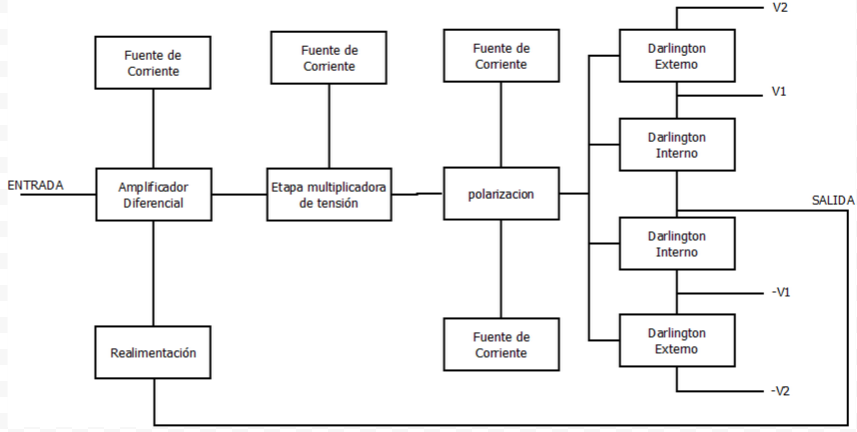
\includegraphics[scale=0.75]{img/ampli_bloques}
	\caption{Diagrama en bloques del amplificador clase G}
	\label{fig:ampli_bloques}
\end{figure}




\subsection{Diseño circuital}

Conseguimos un circuito integrado, especialmente diseñado para audio, que presenta una distorsión considerablemente baja, por lo que decidimos usar este último.
% blablabla


\begin{figure}[H]
\centering
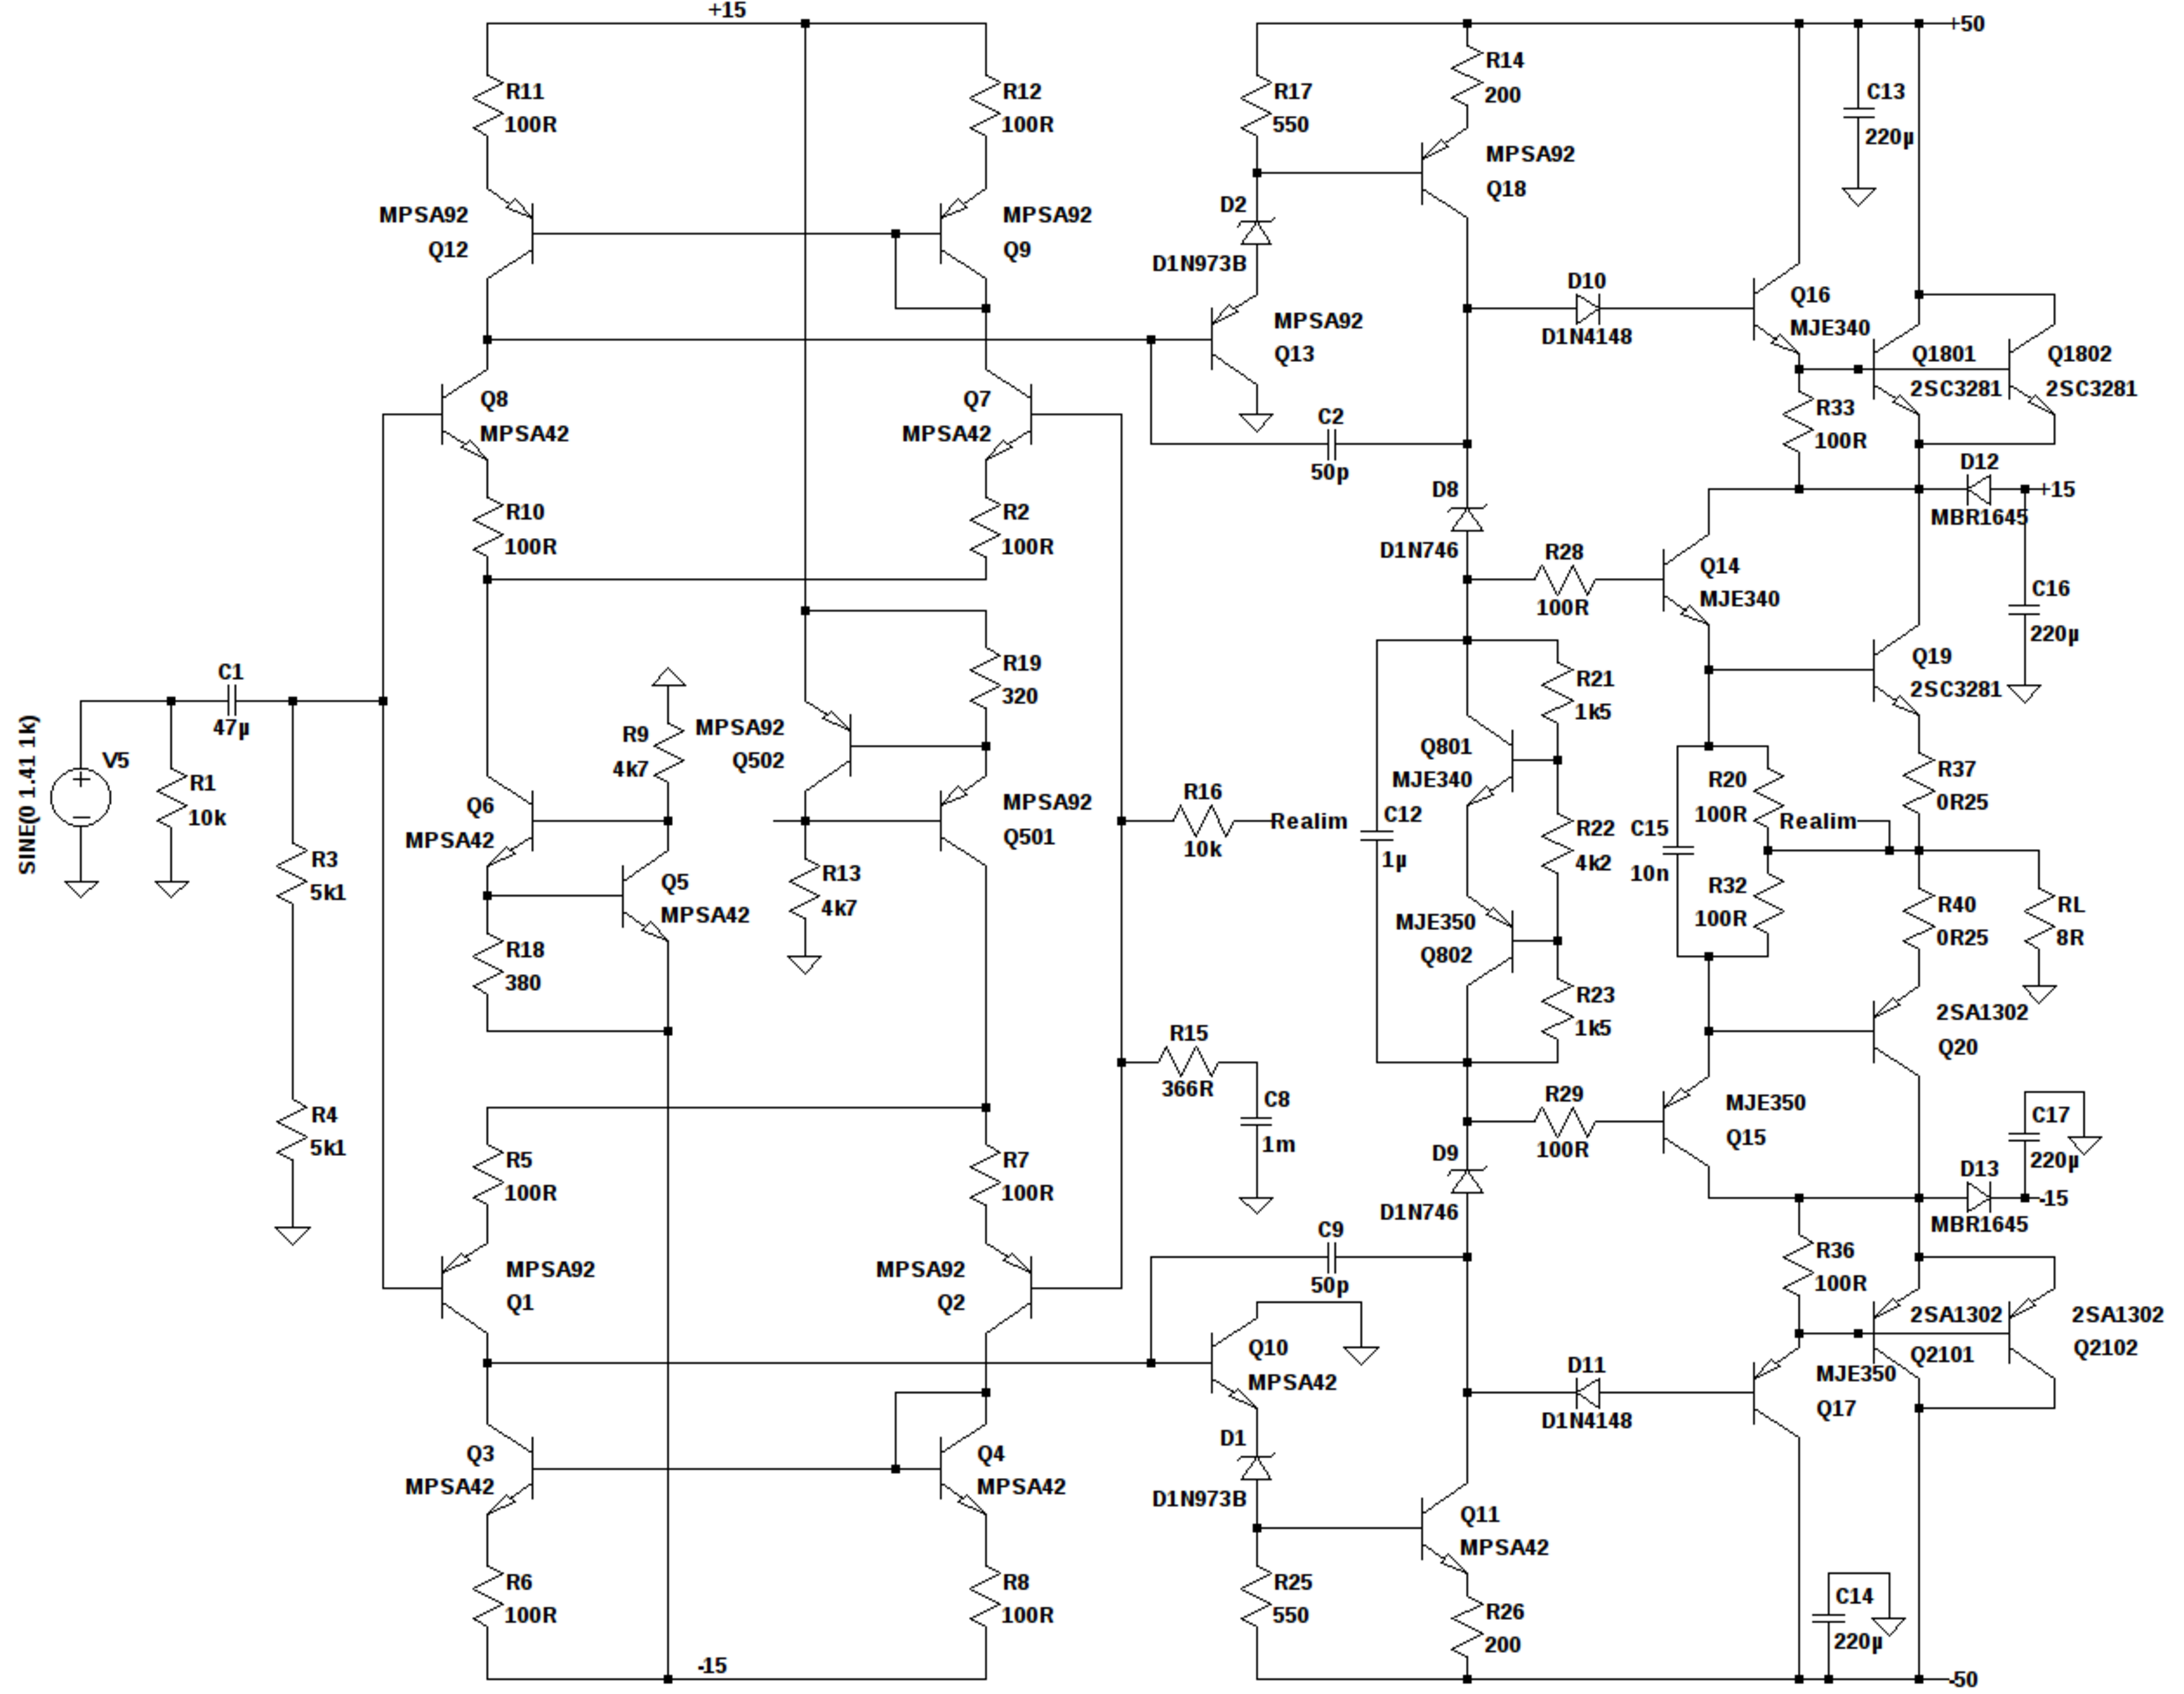
\includegraphics[scale=0.3]{img/circuito.pdf}
\caption{Circuito Diseñado}
\label{circuito} 
\end{figure}

%Dice en la consigna que acá toca:
%1.Explora distintos circuitos y analiza CORRECTAMENTE su funcionamiento*
%2.Calcula CORRECTAMENTE TODOS los componentes de circuitos individuales y las
%condiciones de funcionamiento*
%3.Investiga y selecciona los componentes
%4.Valida y optimiza el diseño mediante simulaciones y mediciones, y determina todos los
%parámetros de funcionamiento de los circuitos
%5.Determina si las especificaciones del circuito son alcanzables*
%6.Realiza las simulaciones, indica y explica los circuitos simulados, los puntos de medición,
%los parámetros utilizados y los resultados obtenidos
%7.Realiza mediciones, indica y explica los circuitos implementados, las mediciones
%realizadas, los instrumentos utilizados y los resultados obtenidos*
%8.Realiza los diagramas esquemáticos con las referencias de todos sus componentes
%9.Realiza el listado de componentes indicando referencia, descripción, valor, parámetros, fabricantes y posibles proveedores para cada componente.

\subsubsection{Simulaciones}

\paragraph{THD para entrada de 1V @ 1kHz} A continuación se muestra una tabla con los resultados del análisis de Fourier realizados con el LTSpice. Se mantuvieron los mismos parámetros de simulación que en la simulación en tiempo.




\begin{verbatim}
Harmonic	Frequency	 Fourier 	Normalized	 Phase  	Normalized

 Number 	  [Hz]   	Component	 Component	[degree]	Phase [deg]

    1   	1.000e+03	2.826e+01	1.000e+00	   -0.03°	    0.00°

    2   	2.000e+03	6.288e-03	2.225e-04	   90.53°	   90.56°

    3   	3.000e+03	7.973e-03	2.821e-04	   -1.25°	   -1.22°

    4   	4.000e+03	9.202e-04	3.256e-05	 -106.33°	 -106.30°

    5   	5.000e+03	3.372e-03	1.193e-04	   -7.83°	   -7.81°

    6   	6.000e+03	7.476e-04	2.645e-05	 -130.81°	 -130.78°

    7   	7.000e+03	9.363e-04	3.313e-05	   20.01°	   20.04°

    8   	8.000e+03	5.653e-04	2.000e-05	   71.66°	   71.69°

    9   	9.000e+03	7.071e-04	2.502e-05	  123.98°	  124.01°

   10   	1.000e+04	9.466e-04	3.349e-05	   45.78°	   45.81°

Total Harmonic Distortion: 0.038514%
\end{verbatim}

La distorsión armónica simulada es de $0.038\%$. % Habría que mejorarla, ¿no?

\paragraph{Slew Rate} Simulando una entrada escalón en el amplificador, se observa la salida de la figura~\ref{fig:slew} en la carga.

La pendiente es de $33 \frac{V}{\mu s}$.


\begin{figure}[H]
	\centering
	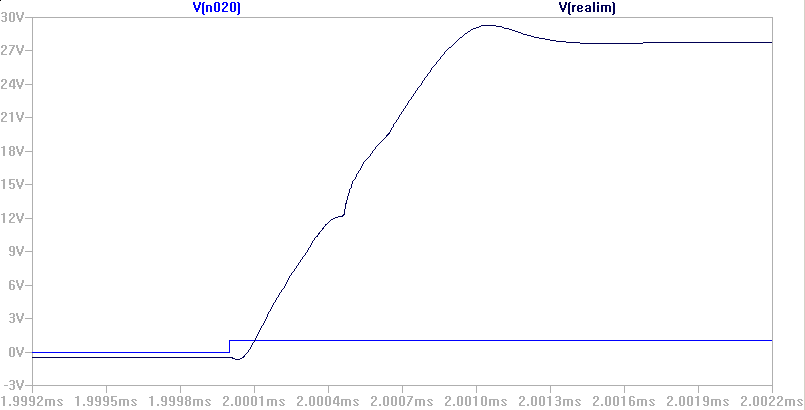
\includegraphics[width=0.8\textwidth]{img/sim/slew}
	\caption{Salida simulada frente a una entrada escalón.}
	\label{fig:slew}
\end{figure}


\paragraph{Resistencia de salida}  

Para la simulación de la resistencia de salida, se obtuvo la tensión pico para una entrada de $0.5V$, con carga de $4\Omega$ ($V_{4\Omega}$)y sin carga ($V_{\infty}$). Se obtiene con la fórmula de divisor de tensión:

\[V_{4\Omega}=V_o \frac{R_L}{R_L+R_{out}}\]
\[R_{out}=R_L \left(\frac{V_{\infty}}{V_{4\Omega}}-1 \right)\]

Se obtuvo:

\[R_{out}\cong 0.01\Omega]\]

La realimentación logra que la resistencia de salida sea muy baja.

\paragraph{Resistencia de entrada}

Se simuló en $1kHz$ el cociente entre la tensión de entrada y la corriente entregadas por el generador.

\[R_{in}=5k\Omega\]

% Parece baja?

\paragraph{Respuesta en frecuencia} 

Se realizó un barrido de $0.1Hz$ a $100MHz$.

\begin{figure}[H]
	\centering
	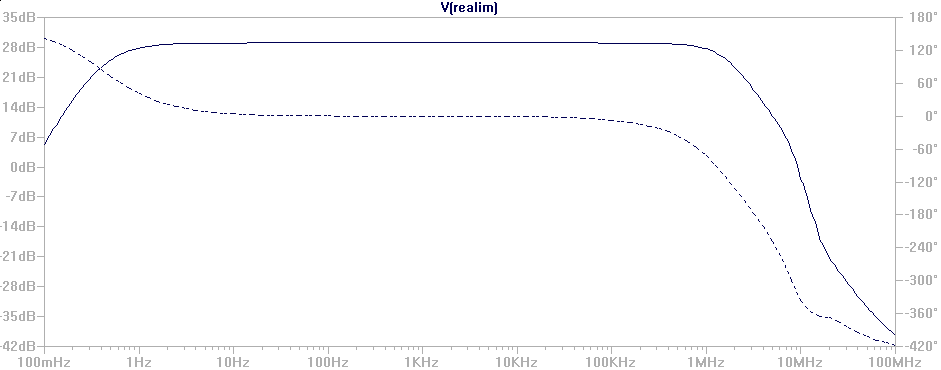
\includegraphics[width=0.8\textwidth]{img/sim/bode}
	\caption{Diagrama de Bode del amplificador a lazo cerrado simulado. El módulo, en línea llena y la fase en línea punteada.}
	\label{fig:bode}
\end{figure}




\paragraph{Ancho de banda de potencia}

\subsection{Análisis de los condicionantes de integración}

%     Requerimientos Eléctricos ( Seguridad eléctrica y 
%Compatibilidad electromagnética), 
%Mecánicos (Vibraciones y Rigidez) y Térmicos (Disip
%ación de los componentes) 

 %    Definición de módulos 

%     Diseño de los Circuitos impresos 

%    Guía de localización de los componentes 

%     Diagrama de conexionado 

%     Dimensionamiento del conexionado 

%     Dimensionamiento y forma de la estructura o gabinete 

%     Dimensionamiento y posición de los puntos de fijación 

%    Diseño de los mecanismos de disipación 

%     Detalles de ensamblado y montaje 

%     Diagramas esquemáticos 

%     Listado de partes  

%     Listado de proveedores 

%     Pruebas funcionales y ambientales 

%     Análisis de modo y efecto de falla de los componentes 

%     Análisis de confiabilidad de los componentes 

%     Optimización 


\subsection{Diseño PCB}


\section{Grado de avance}

Hasta el momento, hemos elegido las configuraciones de las distintas etapas, buscando aquellas que nos provean una menor distorsión; realizamos los cálculos para hallar los valores de realimentación, resistencias para el embalamiento térmico y los disipadores para los transistores; realizamos la simulación del circuito, y estamos en proceso de diseño de la fuente para reducir la tensión de alimentación a un valor apropiado para los integrados que utilizaremos en la primera etapa. 

\section{Dificultades encontradas}

Para el desarrollo del proyecto, nos encontramos con varios obstáculos. En el primer diseño que realizamos, nos encontramos con una disparidad en las corrientes del par diferencial, que resolvimos comprando transistores de más, midiendo sus parámetros $\beta$, y agrupándolos para poder trabajar con valores apareados. Otra solución que encontramos, y que aplicaremos en esta versión del circuito, es utilizar transistores integrados, que asegura que todos los transistores tengan las mismas propiedades, y estén apareados.


\section{Resumen de actividades a desarrollar}

Habiendo establecido todo lo anterior, procederemos con la simulación del circuito con las fuentes switching en la parte diferencial, el diseño del PCB comparte parte con la versión que realizamos el cuatrimestre pasado, por lo que sólo será necesario rediseñar la primera parte. Luego procederemos con el armado del circuito, verificando el correcto funcionamiento de las etapas, durante el armado de la placa, y luego tendremos que revisar que esté andando correctamente, y que cumpla con las parámetros que propusimos. Finalizado esto, procederemos a realizar las mediciones pertinentes.


\end{document}